\section{Background}
\begin{frame}
	\frametitle{Frequency quality in the Nordics}
	\begin{columns}
		\begin{column}{0.5\textwidth}
			\begin{itemize}
				\item<1-> From 2008 there has been a growing concern for power system frequency.
				\item<2-> It is a question of balancing
			\end{itemize}
		\end{column}
		\begin{column}{0.5\textwidth}
			\begin{figure}
				\includegraphics<1>[width=0.8\textwidth]{./pictures/frequency.pdf}
				\includegraphics<2>[width=0.8\textwidth]{./pictures/balance.png}
			\end{figure}
		\end{column}
	\end{columns}
\end{frame}
\begin{frame}
	\frametitle{Why frequency is a question of balance}
	\begin{columns}
		\begin{column}{0.5\textwidth}
					\begin{equation}\label{eq:swing}
				J \dot{\omega}_m +D_d\omega_m = T_m-T_e 
		\end{equation}
		\begin{equation}\label{eq:w_w}
			\omega_e = \frac{p}{2}\omega_m
		\end{equation}
		\begin{itemize}
				\item Most generators are synchronous generators
		\end{itemize}
		\end{column}
		\begin{column}{0.5\textwidth}
			\begin{figure}
				\includegraphics<1>[width=0.8\textwidth]{./pictures/swing.tikz}
			\end{figure}
		\end{column}
	\end{columns}
\end{frame}
\begin{frame}
	\frametitle{Hydro power, the main producer in the Nordic system}
			\begin{figure}
				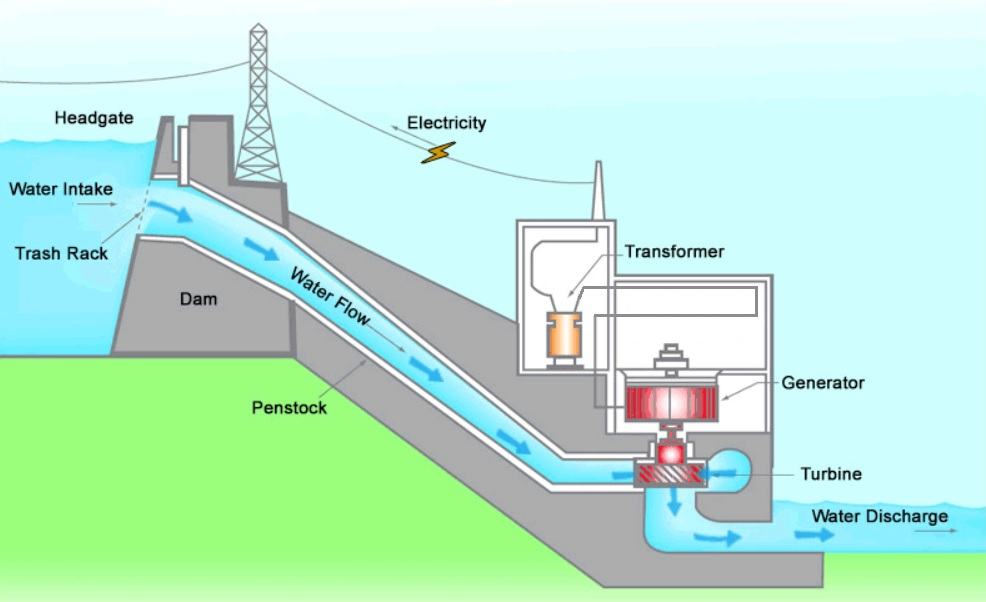
\includegraphics[width=0.8\textwidth]{./pictures/power_plant.png}
		\end{figure}
\end{frame}
\begin{frame}
	\frametitle{Modelling of a hydro power plant}
	\begin{columns}
		\begin{column}{0.3\textwidth}
			\begin{itemize}
				\item Nonlinear
				\item Bernoulli used for derivation
				\item Operates normally within a small operating region
			\end{itemize}
		\end{column}
		\begin{column}{0.7\textwidth}
	\begin{figure}
		\centering
		\includegraphics{./pictures/dam.tikz}
		\includegraphics{./pictures/turbine.tikz}
	\end{figure}
	\end{column}
\end{columns}
\end{frame}
\begin{frame}
	\frametitle{Different frequency control mechanisms}
			\begin{figure}
				\includegraphics<1>[width=0.8\textwidth]{./pictures/balancing.png}
				\includegraphics<2>[width=0.8\textwidth]{./pictures/primary.png}
				\includegraphics<3>[width=0.8\textwidth]{./pictures/fcc.png}
		\end{figure}
\end{frame}
\begin{frame}
	\frametitle{Frequency containment control}
	\begin{itemize}
			\item Each plant has to provide FCC
			\item the amount is given by
				\begin{equation}
						\Delta P_{m1} = G_p(0)\Delta\omega_1
				\end{equation}

	\end{itemize}
		\includegraphics{./pictures/plant_loop.tikz}
\end{frame}
\begin{frame}
	\frametitle{Determining the amount of FCC in the system}
	\begin{itemize}
			\item The maximum allowed frequency deviation is $\pm 0.1Hz$.
			\item The largest power production unit in Norway is $1450MW$.
			\item This gives us
				\begin{equation}
						\sum_i^N G_{pi}(0)=\frac{1450MW}{0.2\pi rad/s}
			\end{equation}
	\end{itemize}
\end{frame}
\begin{frame}
	\frametitle{The industry's response to the frequency quality}
	\begin{itemize}
		\item<1-> Remember the frequency concern?
		\item<2-> Nordic TSOs are developing new requirements for FCR.
		\item<3-> This includes offline testing of hydro power plants.
	\end{itemize}
		\begin{figure}
				\includegraphics<1>[width=0.4\textwidth]{./pictures/frequency}
				\includegraphics<2,3>[width=0.4\textwidth]{./pictures/fcr}
		\end{figure}
\end{frame}
\begin{frame}
	\frametitle{Draft requirements proposed by industry}
	\begin{itemize}
		\item Check the plant's stability margin using the sensitivity function
			\begin{equation}
					S(s)=\frac{1}{1+G_p(s)G_J(s)}
			\end{equation}
		\item Check the disturbance rejection
				\begin{equation}
					G_1(s) = -G_J(s)S(s)
				\end{equation}
		\end{itemize}
\end{frame}
\begin{frame}
	\frametitle{Drawbacks with the draft requirements}
		\begin{itemize}
			\item The plant has to be operated in open loop
			\item Injecting  $10$ sine waves take a lot of time.
			\item They assume the same swing dynamics for all plants.(use same $G_J(s)$ )
	\end{itemize}
	\includegraphics{./pictures/plant_open.tikz}
\end{frame}
\begin{frame}
	\frametitle{Research question}
	\begin{itemize}
		\item Can the draft requirements be tested using PMU measurements from normal operation?
		\item Can we check if the plant's deliver the amount of FCR ($G_p(0)$) as they are supposed to using PMUs?
		\item Or if not what can we say about a power plant's performance using PMU measurements?
\end{itemize}
	\begin{figure}
		\includegraphics{./pictures/genTrafo.tikz}
	\end{figure}
\end{frame}
